\documentclass{beamer}
\usepackage[utf8]{inputenc}
\usepackage{xspace}
\usepackage{hyperref}
\usepackage{listings}
\usepackage{color}
\usepackage{inconsolata}
\usepackage{tikz}
\usetikzlibrary{fadings}

\usepackage{templates/beamerthemekit}
\usepackage{pdfpcnotes}

\lstdefinestyle{c}{language=C,
basicstyle=\footnotesize\ttfamily,
commentstyle=\color{green},
%identifierstyle=\color{blue},
keywordstyle=\color{purple},
stringstyle=\color{cyan}
}

\setbeamercovered{invisible}

\titleimage{AhmadinejadNatanz_cropped_caption}

\title{Stuxnet}
\subtitle{Proseminar: Desaster in der Software-Sicherheit}
\author{Lucas Werkmeister}
\date{Januar / Februar 2015}

\begin{document}

\begin{frame}
  \titlepage
  \pnote{Begruessung}
\end{frame}

%\begin{frame}
%  \tableofcontents
%  \pnote{Gliederung}
%\end{frame}

\section{Einführung}

\subsection{Allgemeines}

\begin{frame}
  \frametitle{Allgemeines}
  \begin{itemize}
    \item Computerwurm, zwei Versionen:
      \begin{itemize}
        \item 0.5: 2007-2009
        \item 1.x: 2010
      \end{itemize}
    \item Gezielter Angriff auf iranische Uran-Anreicherungsanlage
    \item Geschätzter Entwicklungsaufwand: ca.~10~Entwickler, 6~Monate + Quality Assurance, Testen, etc.
    \item Testen erfordert Nachbau der Anlage (inkl. echtes Uran)
    \item Folgerung: Staatliche Angreifer (Annahme: USA)
  \end{itemize}
  \pnote{Hinweise (myrtus) erwaehnen, Tasten im Nebel, nicht drauf eingehen}
\end{frame}

\subsection{Urananreicherung}

\begin{frame}
  \frametitle{Urananreicherung}
  \begin{itemize}
    \item Gaszentrifugen: Gas mit schwererem Uran sammelt sich außen
    \item Sehr niedriger Druck: ca.~2-5~mbar (TKaC 26)
    \item Höhere Frequenzen: Stärkere Anreicherung, aber instabiler
    \item Im Iran: IR-1-Zentrifuge – europäisches Modell der 60er/70er
      \begin{itemize}
        \item ``obsolete design that Iran never managed to operate reliably'' (TKaC 5)
        \item Häufige Ausfälle trotz verringertem Betriebsdruck
        \item Dafür: Massenproduktion
      \end{itemize}
  \end{itemize}
  \pnote{UF6 wird bei 100mbar fest (TKaC 7)\\IR-1: Best case: nur halbe theoretische Ausbeute}
\end{frame}

\section{Physische Angriffe}

\subsection{Steuerung der Anlage}

\begin{frame}
  \frametitle{Steuerung der Anlage}
  \begin{itemize}
    \item Anlagensteuerung durch SCADA-Software, z.~B. WinCC
    \item Irans SCADA-Software: Unbekannt, offenbar Eigenbau
      \begin{itemize}
        \item ``quite amateurish by Western standards […] custom-built […] little familiarity with contemporary SCADA software design'' (TKaC 27)
        \item Aber durchgehend Englisch, selbst mit US-Datumsformat
      \end{itemize}
    \item Direkte Steuerung erfolgt über \emph{Programmable Logic Controllers}~(PLCs)
      \begin{itemize}
        \item S7-417: Ventile und Drucksensoren (1.~Angriff)
        \item S7-315: Rotoren (2.~Angriff)
      \end{itemize}
    \item PLCs werden mit \emph{Step7} programmiert
  \end{itemize}
  \pnote{SCADA: Nur ein unwichtiges Farsi-Label gesehen}
\end{frame}

\subsection{1. Angriff: Stuxnet 0.5}

\begin{frame}
  \frametitle{1. Angriff: Stuxnet 0.5}
  \begin{itemize}
    \item Manipulation der Ventile an den Zentrifugen
    \item Überdruck in den Zentrifugen
    \item Während des Angriffs werden alte Sensordaten abgespielt
    \item Angriff endet \emph{bevor} irreparabler Schaden entsteht
  \end{itemize}
  \pnote{Dampfkochtopf-Analogie?\\21 Sekunden replay\\bei Pressure controllers, die Dump Line kontrollieren, wird Linearisierungs-Kalibrierung ueberschossen\\Erinnerung: 2-5mbar Betriebsdruck, fest bei 100mbar}
\end{frame}

\subsection{2. Angriff: Stuxnet 1.x}

\begin{frame}
  \frametitle{2. Angriff: Stuxnet 1.x}
  \begin{itemize}
    \item Manipulation der Rotorgeschwindigkeit
      \begin{itemize}
        \item Normale Betriebsgeschwindigkeit: 63000rpm (1050Hz)
        \item Erhöhte Geschwindigkeit: 84600rpm (1410Hz)
        \item Verringerte Geschwindigkeit: 120rpm (2Hz)
      \end{itemize}
    \item Leicht festzustellen (zuhören) – insbesondere, wenn synchronisiert
  \end{itemize}
  \pnote{Es werden NICHT alte Sensordaten abgespielt! Unnoetig: Konst. Geschw. erwartet, ausserdem SCADA liest Daten aus Speicher, nicht direkt aus Geraet.\\Angriff wurde via WinCC synchronisiert (unklar ob im Iran verwendet), noch leichter zu hoeren}
\end{frame}

\section{IT-Angriffe}

\subsection{Verbreitung}

\begin{frame}
  \frametitle{Verbreitung}
  \begin{itemize}
    \item Step7-Projekte: Infektion der Step7-Installation beim Öffnen von infizierter Datei
    \item Memory Sticks:
      \begin{itemize}
        \item \texttt{autorun.inf}: Infektion von Windows bei Autorun oder manuellem Öffnen (Version~1.001)
        \item \texttt{.lnk}-Dateien: Infektion von Windows beim Öffnen im Explorer (Versionen~1.10x)
      \end{itemize}
    \item Netzwerk
      \begin{itemize}
        \item WinCC: Infektion des Servers, wenn möglich (Versionen~1.x)
        \item SMB: Infektion des Remote-Systems, wenn möglich (Versionen~1.x)
        \item Print Spooler: Infektion des Remote-Systems, wenn möglich (Versionen~1.x)
      \end{itemize}
  \end{itemize}
  \pnote{Beachte: 0.5 nur Step7}
\end{frame}

\subsection{Updates}

\begin{frame}
  \frametitle{Updates}
  \begin{itemize}
    \item Command and Control-Server: Rückmeldung, dann neue Executable herunterladen und ausführen
      \begin{itemize}
        \item 0.5: \url{smartclick.com}, \url{best-advertising.net}, \url{internetadvertising4u.com}, \url{ad-marketing.net}
        \item 1.x: \url{www.mypremierfutbol.com}, \url{www.todaysfutbol.com}
      \end{itemize}
    \item Peer-to-Peer Updates
      \begin{itemize}
        \item Bei jeder Neuinfektion wird zunächst auf eine vorhandene Version geprüft und, falls vorhanden, die ältere aktualisiert
        \item 0.5: Windows mailslots, file shares
        \item 1.x: RPC server + client
      \end{itemize}
  \end{itemize}
  \pnote{Domains mittlerweile alle Besitzer gewechselt\\RPC = Remote Procedure Call\\Mailslots: InterProcess Communication Mechanismus, über RPC, einfach gehalten}
\end{frame}

\subsection{CVE-2010-2743}

\begin{frame}
  \frametitle{CVE-2010-2743 Local Privilege Escalation (1.10x)}
  \begin{itemize}
    \item \texttt{win32k.sys} lädt Keyboard-Layouts, läuft im Kernel-Mode
    \item Ein Index in eine Funktionspointer-Tabelle wird nicht korrekt verifiziert
    \item Stuxnet weist Windows an, eine nicht wohlgeformte Keyboard-Layout-Datei zu laden
    \item Dadurch wird Stuxnet-Code im Kernel-Mode ausgeführt
  \end{itemize}
  \pnote{0-day-exploit\\CVE = Common Vulnerabilities and Exposures}
\end{frame}

\begin{frame}
  \frametitle{Function Table}
  \lstinputlisting[language=C,style=c]{../functionPointerDemo/01-harmless.c}
  \pnote{Was passiert mit Index 2?}
\end{frame}

\begin{frame}
  \frametitle{Absturz}
  \lstinputlisting[language=C,style=c]{../functionPointerDemo/02-broken.c}
  \pnote{Segfault.\\nm zeigt: table ganz am ende, danach nur __TMC_END__.}
\end{frame}

\begin{frame}
  \frametitle{Infektion}
  \lstinputlisting[language=C,style=c]{../functionPointerDemo/03-infected.c}
  \pnote{nm zeigt: table1, table2, __TMC_END__.}
\end{frame}

\begin{frame}
  \frametitle{Absicherung}
  \lstinputlisting[language=C,style=c]{../functionPointerDemo/04-protected.c}
  \pnote{echter code: bessere fehlerbehandlung\\sizeof(table)/sizeof(table[0])}
\end{frame}

\subsection{CVE-2012-3015}

\begin{frame}
  \frametitle{CVE-2012-3015 Step7-Infektion (alle Stuxnet-Versionen)}
  \begin{itemize}
    \item Step7 lädt DLLs; Search Path kann in der Config-Datei manipuliert werden, um DLLs innerhalb des Projektordners zu enthalten
    \item Verschiedene Funktionen (z.~B. Blöcke schreiben und lesen) werden von Stuxnet-DLL bereitgestellt
    \item Behoben dadurch, dass DLLs in Projektordnern nicht verwendet werden (SSA-110665)
  \end{itemize}
  \pnote{Untrusted Search Path Vulnerability}
\end{frame}

\section{Vergleich}

\subsection{Stuxnet 0.5 und 1.x: Verbreitung}

\begin{frame}
  \frametitle{Stuxnet 0.5 und 1.x: Verbreitung}
  \begin{itemize}
    \item Stuxnet 0.5
      \begin{itemize}
        %\item Sehr zielgerichteter und komplexer Angriff
        \item Sehr eingeschränkte Verbreitung: Ausschließlich Step7-Infektionen
      \end{itemize}
    \item Stuxnet 1.x
      \begin{itemize}
        %\item Einfacherer Angriff
        \item Breite Vielfalt an Verbreitungsmethoden, einschließlich 4~Zero-Day-Exploits
        \item Größerer Aufwand, höheres Entdeckungsrisiko; warum?
      \end{itemize}
  \end{itemize}
  \only<1>{
    \begin{figure}[p]
      \centering
      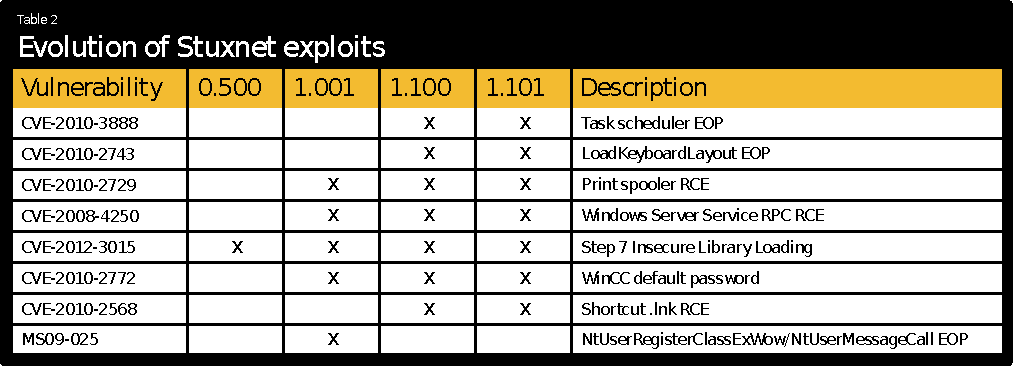
\includegraphics[height=0.35\textheight]{../Evolution_exploits.pdf}
      
      \tiny{Quelle: Symantec Security Response, Stuxnet 0.5: The Missing Link, S.~2}
    \end{figure}
  }
  \only<2>{
    \begin{figure}[p]
      \centering
      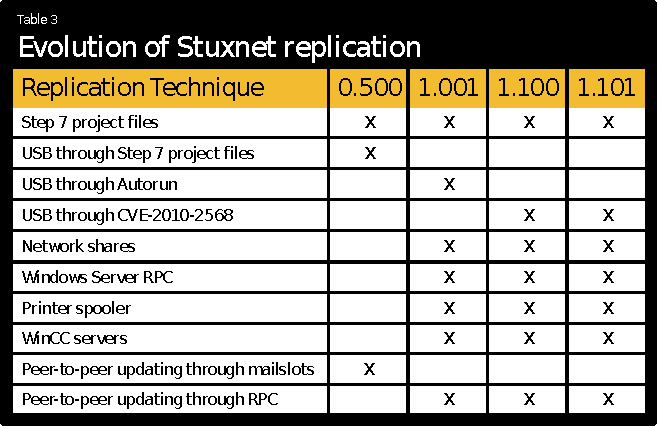
\includegraphics[height=0.35\textheight]{../Evolution_replication.pdf}
      
      \tiny{Quelle: Symantec Security Response, Stuxnet 0.5: The Missing Link, S.~2}
    \end{figure}
  }
\end{frame}

\subsection{Defense in Depth}

\begin{frame}
  \frametitle{Defense in Depth}
  \begin{itemize}
    \item Angreifer durch weit ausgedehnte Verteidigung schwächen
    \item In IT: Mehrere, redundante Sicherheits-Ebenen
    \item Vollständiger Angriff wird erschwert und kann über längeren Zeitraum besser bemerkt werden
  \end{itemize}
\end{frame}

\subsection{Ursache der unterschiedlichen Verbreitung}

\begin{frame}
  \frametitle{Ursache der unterschiedlichen Verbreitung}
  \begin{itemize}
    \item<1-> Stuxnet 0.5 kam mit nur einer Verbreitungsmethode ans Ziel
      \begin{itemize}
        \item Vermutlich durch Subunternehmer eingebracht
        % TODO remove the following item? verbal only?
        \item Entwicklung benötigte auch detaillierte Informationen über Anlage:
          ``whoever provided the required intelligence may as well know the favorite pizza toppings of the local head of engineering'' (TKaC 10)
      \end{itemize}
      \begin{itemize} % causes pdfpc to crash if put into the previous itemize
        \item Weiteres Beispiel von Sicherheitslücke durch Subunternehmer? \pause Edward Snowden
      \end{itemize}
    \item<3-> Stuxnet 1.x benötigte mehrstufige Verbreitung
      \begin{itemize}
        \item Zugangsweg von 0.5 vermutlich nicht mehr verfügbar
        \item Stuxnet 1.x musste sich ``durchhangeln''
      \end{itemize}
  \end{itemize}
  \pnote{Snowden: Booz Allen Hamilton; Sysadmin bei NSA, über sämtlichen Clearance-Stufen}
\end{frame}

\section{Abschluss}

\subsection{Erfolg von Defense in Depth}

\begin{frame}
  \frametitle{Erfolg von Defense in Depth}
  \centering
  \resizebox{!}{0.75\textheight}{
    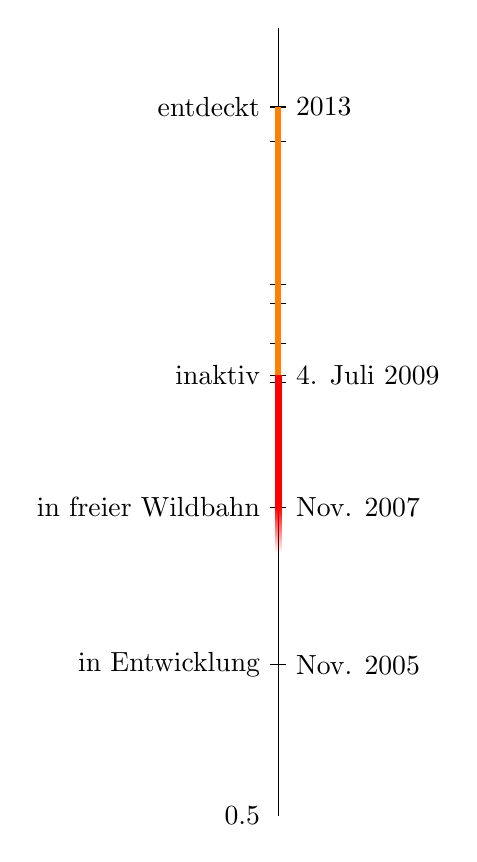
\begin{tikzpicture}[]
      \draw (0,0) -- (0,120/12);
      
      \foreach \x in {23, 47, 67.13, 108, 66, 72, 78, 81, 102.8}{
        \draw (3pt,\x/12) -- (-3pt,\x/12);
      }
      
      \draw (0,0/12) node[left=3pt] { 0.5 };
      \draw (0,23/12) node[left=3pt] { in Entwicklung } node[right=3pt] { Nov. 2005 };
      \draw (0,47/12) node[left=3pt] { in freier Wildbahn } node[right=3pt] { Nov. 2007 };
      \draw (0,67.13/12) node[left=3pt] { inaktiv } node[right=3pt] { 4. Juli 2009 };
      \draw (0,108/12) node[left=3pt] { entdeckt } node[right=3pt] { 2013 };

      \draw [orange, line width = 2pt] (0,67.13/12) -- (0,108/12);
      \fill [red, path fading = south] (-1.25pt,40/12) -- (-1.25pt,47/12) -- (1.25pt,47/12) -- (1.25pt,40/12) -- cycle;
      \draw [red, line width = 2.5pt] (0,47/12) -- (0,67.13/12);
    \end{tikzpicture}
  }
  \resizebox{!}{0.75\textheight}{
    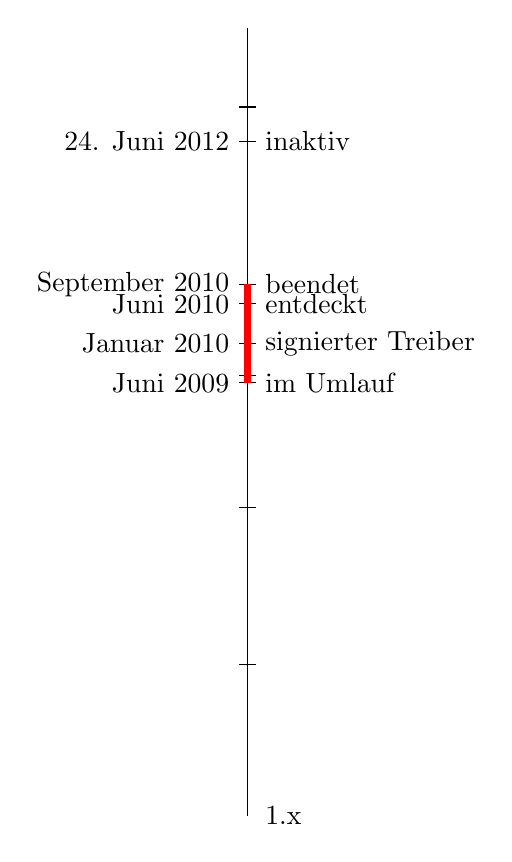
\begin{tikzpicture}[]
      \draw (0,0) -- (0,120/12);
      
      \foreach \x in {23, 47, 67.13, 108, 66, 72, 78, 81, 102.8}{
        \draw (3pt,\x/12) -- (-3pt,\x/12);
      }
      
      \draw (0,0/12) node[right=3pt] { 1.x };
      \draw (0,66/12) node[right=3pt] { im Umlauf } node[left=3pt] { Juni 2009 };
      \draw (0,72/12) node[right=3pt] { signierter Treiber } node[left=3pt] { Januar 2010 };
      \draw (0,78/12) node[right=3pt] { entdeckt } node[left=3pt] { Juni 2010 };
      %\draw (0,79/12) node[right=3pt] { mehr Signaturen } node[left=3pt] { Juli 2010 };
      \draw (0,81/12) node[right=3pt] { beendet } node[left=3pt] { September 2010 };
      \draw (0,102.8/12) node[right=3pt] { inaktiv } node[left=3pt] { 24. Juni 2012 };
      
      \draw [red, line width = 2.5pt] (0,66/12) -- (0,81/12);
    \end{tikzpicture}
  }
  \pnote{2005: Domain registriert\\Beachte: 1.x vor Entdeckung im Umlauf, 2007 vmtl zu spät}
\end{frame}

\subsection{Quellen}

\begin{frame}
  \frametitle{Quellen}
  \fontsize{6pt}{7.2}\selectfont
  \begin{itemize}
    \item Dossier: Symantec Security Response, W32.Stuxnet Dossier, \url{https://www.symantec.com/content/en/us/enterprise/media/security_response/whitepapers/w32_stuxnet_dossier.pdf}
    \item 0.5: Symantec Security Response, Stuxnet 0.5: The Missing Link, \url{https://www.symantec.com/content/en/us/enterprise/media/security_response/whitepapers/stuxnet_0_5_the_missing_link.pdf}
    \item TKaC: Ralph Langner, To Kill a Centrifuge, \url{http://www.langner.com/en/wp-content/uploads/2013/11/To-kill-a-centrifuge.pdf}
    \item CVE-2010-2743: \url{https://cve.mitre.org/cgi-bin/cvename.cgi?name=CVE-2010-2743}
    \item CVE-2012-3015: \url{https://cve.mitre.org/cgi-bin/cvename.cgi?name=CVE-2012-3015}
    \item SSA-110665: \url{https://www.siemens.com/innovation/pool/de/forschungsfelder/siemens_security_advisory_ssa-110665.pdf}
    \item Diese Folien sind auch verfügbar unter \url{https://github.com/lucaswerkmeister/Proseminar-Stuxnet}.
  \end{itemize}
  \pnote{Weg damit}
\end{frame}

\end{document}
